Athena uses a number of unit tests during the development lifecycle to ensure core I/O functionality does not break.
Many of the I/O tests were originally created for the old EDM and haven't been updated to test the xAOD EDMs core I/O functions.
The new software developed in this project takes in track information from a unit test using the T/P EDM, writes the data into an example xAOD object to file and reads it back.


\section{xAOD Test Object}
\label{sec:Mod_utests_xAOD_object}

% Overview
The object used to employ the new unit test is the \verb|xAOD::ExampleElectron| object, where the \verb|xAOD::| is a declaration of the namespace and simply identifies the object as an xAOD object.
An individual \verb|ExampleElectron| object only has a few parameters for sake of testing, its transvese momentum, \verb|pt|, and its charge, \verb|charge|.
A collection of \verb|ExampleElectron| objects are stored in the \verb|ExampleElectronContainer| object, which is just a \verb|DataVector| of \verb|ExampleElectron| objects.\cite{Buckley_2015}
This \verb|DataVector| acts similar to an \verb|std::vector|. 
 
% Explain Aux Store better
The xAOD EDM utilizes a separation between between static and dynamic data stores.

The static data stores comprise variables directly attributed to the object associated with it, the dynamic counterpart stores data of variables added by the user.
An example of a static variable might be an electrons transverse momenta or its charge, while an example of a dynamic attribute might be a link associating that object with a specific track.  


Figure \ref{fig:Mod_utests_aux_store} illustrates how a simple setup of storing a \verb|DataVector| of electrons that hold some specific parameters into one \verb|IAuxStore| while also having a separate \verb|IAuxStore| specifically for the dynamic attributes. 

\begin{figure}[h]
    \centering
    \vspace{20px}
    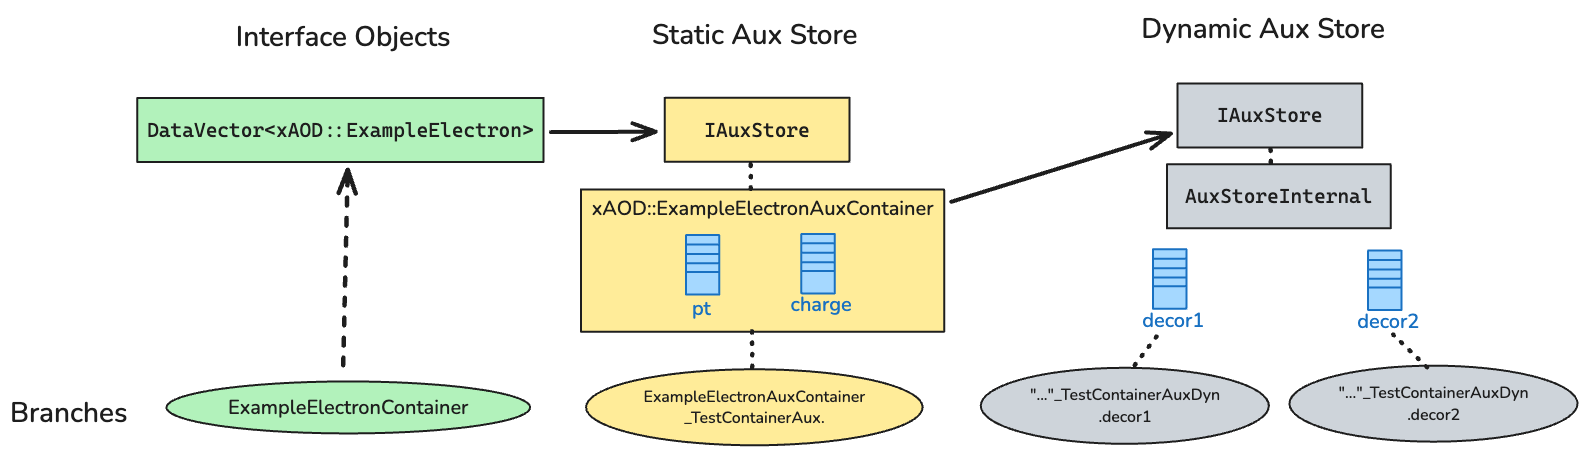
\includegraphics[width=\textwidth]{content/img/aux_store_better.png}
    \caption{The framework between interface objects and the static/dynamic auxiliary data store for a collection of xAOD::ExampleElectrons.}
    \label{fig:Mod_utests_aux_store}
\end{figure}





\section{Unit Tests}
\label{sec:Mod_utests_CI}
Unit tests are programs that act as a catch during the continuous integration of a codebase and test features that need to remain functional. 
Athena has a number of unit tests that check every merge request and nightly build for issues in the new code that could break core functionality, either at the level of Athena, ROOT, or any other software in the LCG stack.
There were no unit tests in the appropriate packages to handle selection of dynamic attributes, or decorations, on xAOD objects created during writing and read back.
To address this, a new xAOD test object needed to be created and written during a new unit test that fit into the existing unit tests.
The list of AthenaPoolExample unit tests that are currently executed during a nightly build can be found in Table \ref{tab:CI_Unit_Tests}.
These tests are executed in this order, as the objects created in one might be used in proceeding test.

\begin{table}[h]
    \centering
    \caption{List of unit tests in the AthenaPoolExample package that are currently executed during a nightly build. The unit tests marked by the `*' are the tests produced for this thesis.}
    \label{tab:CI_Unit_Tests}
    \resizebox{\textwidth}{!}{
    \begin{tabular}{|c|c|c|}
        \hline
        $\textbf{Unit Test}$ & $\textbf{Employed Algorithms}$ & $\textbf{Function} (\text{Object Read}) \left[\text{Object Written}\right]$ \\
        \hline
      Write & WriteData & $\left[\text{ExampleHit}\right]$\\
        \hline
        ReadWrite & ReadData, ReWriteData & ($\text{ExampleHit}$), $\left[\text{ExampleTrack}\right]$\\
        \hline
        Read & ReadData & ($\text{ExampleHit}$)\\
        \hline
        Copy & None & $\textbf{Copies a file}$\\
        \hline
        ReadWriteNext & ReadData, ReWriteData & ($\text{ExampleHit}$, EventInfo), $\left[\text{ExampleTrack}\right]$ \\
        \hline
      *WritexAODElectron & ReadData, WriteExampleElectron & ($\text{ExampleTrack}$), $\left[xAOD::ExampleElectrons, decorations \right]$ \\
        \hline
        *ReadxAODElectron & ReadExampleElectron & (xAOD::ExampleElectrons, decorations) \\
        \hline
    \end{tabular}
    }
\end{table}

The mechanism for passing a unit test is done automatically by building the framework, running the unit tests, and comparing the diff of the output file to the unit test with a reference file associated with that particular unit test. 
If the unit test passes, then the diff, a product of the \verb|git diff| command, will be empty and the unit test will be marked as passing.
Conversely, if the unit test fails, then the diff will be non-empty and the unit test will be marked as failing.

\subsection{WritexAODElectron.py}
The two new tests added to the package were \verb|WritexAODElectron| and \verb|ReadxAODElectron|.
During this first unit test, the first algorithm called is to \verb|ReadData| which reads off all of the \verb|ExampleTrack| objects stored in one of the files produced by the \verb|ReadWrite| unit-test.
Within the python script of the first unit test, the user is able to decide what decorations to have written to file. 
This is a part of the \verb|OutputStreamCfg| parameter, \verb|ItemList|, wherein the user specifies the object and its name in the format shown in Figure \ref{fig:Mod_utests_WritexAODElectron_ItemList}. 
\begin{figure}[h]
\centering
\begin{lstlisting}[language=C]
ItemList = [ "ExampleTrackContainer#MyTracks", 
"xAOD::ExampleElectronContainer#TestContainer",
"xAOD::ExampleElectronAuxContainer#TestContainerAux.-decor2"] )
\end{lstlisting}
\caption{WritexAODElectron ItemList for the OutputStreamCfg parameter. Showing how to select dynamic attributes at the CA level.}
\label{fig:Mod_utests_WritexAODElectron_ItemList}
\end{figure}



%% WriteExampleElectronAlgorithm
% Header (.h)
% Much of the code in Athena practice header/source-file separation, the header acting as an interface for the whole object and the source file containing the core functionality of the algorithm.
The header file includes various packages needed by the algorithm, such as data objects, \verb|Write/ReadHandleKeys|, base algorithms that give consistent structure to the algorithm, and whatever else is required. 
In the write-algorithm, there are \verb|ReadHandleKeys| for \verb|ExampleTrack| objects saved by a prior unit test. 
For the \verb|WriteHandleKeys|, there is one for the \verb|ExampleElectronContainer| and the name given to it is ``TestContainer". 
This ``TestContainer" name will be needed for the \verb|ReadExampleElectron| algorithm as the name is how it's able to refer to the correct \verb|ExampleElectronContainer| present in the input file. 
Additionally, a \verb|WriteHandleDecorKey| for the decoration objects is needed for appending each decoration onto each \verb|ExampleElectron| object. 
Figure \ref{fig:Mod_utests_WritexAODElectron_header} shows the syntax for how these keys would be presently defined.

\begin{figure}[h]
\centering
\begin{lstlisting}[language=C]
// Read key ExampleTracks
SG::ReadHandleKey<ExampleTrackContainer> m_exampleTrackKey{
    this, "ExampleTrackKey", "MyTracks"};  

// Write key for the ExampleElectronContainer
SG::WriteHandleKey<xAOD::ExampleElectronContainer>
    m_exampleElectronContainerKey{this, "ExampleElectronContainerName",
                                "TestContainer"};

// Decoration keys
SG::WriteDecorHandleKey<xAOD::ExampleElectronContainer> m_decor1Key{
    this, "ExampleElectronContainerDecorKey1", "TestContainer.decor1",
    "decorator1 key"};
SG::WriteDecorHandleKey<xAOD::ExampleElectronContainer> m_decor2Key{
    this, "ExampleElectronContainerDecorKey2", "TestContainer.decor2",
    "decorator2 key"};
\end{lstlisting}
\caption{WriteExampleElectronheader file setup}
\label{fig:Mod_utests_WritexAODElectron_header}
\end{figure}

% Source File (.c)
Then the \verb|WriteExampleElectron| algorithm is called and takes \verb|ExampleTracks|, creates an \verb|ExampleElectron| object and sets the electrons \verb|pt| to the tracks \verb|pt|. 
\begin{figure}[h]
\centering
\begin{lstlisting}[language=C]
auto elecCont = std::make_unique<xAOD::ExampleElectronContainer>();
auto elecStore = std::make_unique<xAOD::ExampleElectronAuxContainer>();
elecCont->setStore(elecStore.get());

SG::ReadHandle<ExampleTrackContainer> trackCont(m_exampleTrackKey, ctx);
elecCont->push_back(std::make_unique<xAOD::ExampleElectron>());

for (const ExampleTrack* track : *trackCont) {
    // Take on the pT of the track
    elecCont->back()->setPt(track->getPT());
}

SG::WriteHandle<xAOD::ExampleElectronContainer> objs(m_exampleElectronContainerKey, ctx);
ATH_CHECK(objs.record(std::move(elecCont), std::move(elecStore)));
\end{lstlisting}
\caption{Algorithm to initialize and write T/P data (ExampleTracks) to an xAOD object container (ExampleElectronContainer).}
\label{fig:Mod_utests_WritexAODElectron1}
\end{figure}
As shown in Figure \ref{fig:Mod_utests_WritexAODElectron1}, the \verb|ExampleElectronContainer| and \verb|ExampleElectronAuxContainer| are created and set to the \verb|elecCont| and \verb|elecStore| respectively.
The \verb|elecCont| has an associated aux store, so the \verb|setStore| function is called with the \verb|elecStore| pointer.
The track container is accessed by using StoreGate's \verb|ReadHandle|, which associates the \verb|m_exampleTrackKey| with the \verb|ExampleTrackContainer| specified in the header file.
This is then looped over all elements in the container and the \verb|pt| of each track is set to the \verb|pt| of the electron.
A \verb|WriteHandle|, called \verb|objs|, is then created for the container of \verb|ExampleElectrons| which is then recorded.

Within the same algorithm, the next step is to loop over each of the newly produced \verb|ExampleElectrons|, accessing the decorations \verb|decor1| and \verb|decor2|, and setting each to an arbitrary float value that are easily identifiable later.
Figure \ref{fig:Mod_utests_WritexAODElectron2} shows how this is done using two handles for each decoration. 
Note the difference here using the \verb|WriteDecorHandle|, where the prior handle type was \verb|WriteHandle|.
\begin{figure}[h]
    \centering
\begin{lstlisting}[language=C]
SG::WriteDecorHandle<xAOD::ExampleElectronContainer, float> hdl1(m_decor1Key,ctx);
SG::WriteDecorHandle<xAOD::ExampleElectronContainer, float> hdl2(m_decor2Key,ctx);

for (const xAOD::ExampleElectron* obj : *objs) {
    hdl1(objs) = 123.;
    hdl2(objs) = 456.;
}
\end{lstlisting}
    \caption{Writing of dynamic variables for each of the ExampleElectron objects.}
    \label{fig:Mod_utests_WritexAODElectron2}
\end{figure}


\subsection{ReadxAODElectron.py}
The only algorithm called in this test is \verb|ReadExampleElectron|.
The header file for the \verb|ReadExampleElectron| only creates \verb|ReadHandleKey| for the container of ExampleElectrons, with the same name from the header of the \verb|WriteExampleElectron| algorithm header, syntax shown in Figure \ref{fig:Mod_utests_ReadxAODElectron1}.
\begin{figure}[h]
    \centering
\begin{lstlisting}[language=C]
SG::ReadHandleKey<xAOD::ExampleElectronContainer>
m_exampleElectronContainerKey{this, "ExampleElectronContainerName",
                                "TestContainer"};
\end{lstlisting}
    \caption{ReadHandleKey for the container of ExampleElectrons}
    \label{fig:Mod_utests_ReadxAODElectron1}
\end{figure}
From the source file, we can initialize the \verb|ReadHandleKey| object by a simple \verb|ATH_CHECK(m_exampleElectronContainerKey.initialize());| in the \verb|initialize()| method.
This allows for, when defining the \verb|ReadHandle| in execute, identifying the correct container defined in the header file.
The same can be done for the decoration key, which needs a separate read handle, \verb|ReadDecorHandle|. 
Once this is setup, all the read algorithm needs to do is to loop over all the \verb|ExampleElectrons| in the ``TestContainer" and access their $p_T$ and charge.

\section{Results}
This project sought to replace existing unit tests that created \verb|ExampleHits|, T/P EDM objects, to be written and read back. 
An independent xAOD object, \verb|ExampleElectron|, was created and implemented into two new unit tests that write and read \verb|ExampleElectron| objects along with their chosen dynamic attributes. 
A merge request was created, approved, and merged into the Athena software framework.
Future work can be done to fully modernize the package these unit tests reside, \verb|AthenaPoolExampleAlgorithms|, including unit tests that test core functionality of AthenaMT/AthenaMP, and newer storage formats like RNTuple. 
